\documentclass[border=3pt,tikz]{standalone}
\usepackage{amsmath} % for aligned
\usepackage{listofitems} % for \readlist to create arrays
\usetikzlibrary{arrows.meta} % for arrow size
\usepackage[outline]{contour} % glow around text
\contourlength{1.4pt}
\usepackage{tikz-3dplot}

% COLORS
\usepackage{xcolor}
\colorlet{myred}{red!80!black}
\colorlet{myblue}{blue!80!black}
\colorlet{mybluee}{myblue!80!black}
\colorlet{mygreen}{green!60!black}
\colorlet{myorange}{orange!70!red!60!black}
\colorlet{mydarkred}{red!30!black}
\colorlet{mydarkblue}{blue!40!black}
\colorlet{mydarkgreen}{green!30!black}

% STYLES
\tikzset{
  >=latex, % for default LaTeX arrow head
  node/.style={thick,circle,draw=myblue,minimum size=22,inner sep=0.5,outer sep=0.6},
  node in/.style={node,blue!20!black,draw=myblue!30!black,fill=myblue!20},
}
\def\nstyle{int(\lay<\Nnodlen?min(2,\lay):3)} % map layer number onto 1, 2, or 3

\begin{document}

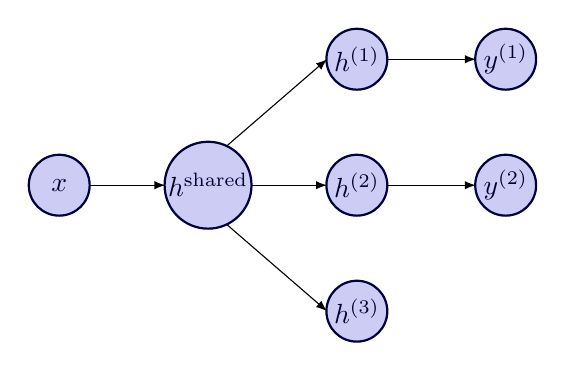
\begin{tikzpicture}[x=2.7cm,y=1.6cm]
  \draw[->] (0.14, 0) -- (0.50, 0) node[pos=0.50] {};
  \node[node in] (0, 0) at (0, 0) {$x$};
  \draw[->] (0.84, 0) -- (1.26, 0) node[pos=0.50] {};
  \draw[->] (0.78, 0.3) -- (1.26, 1) node[pos=0.50] {};  
  \draw[->] (0.78, -0.3) -- (1.26, -1) node[pos=0.50] {};  
  \node[node in] (0, 0) at (0.7, 0) {$h^\text{shared}$};
  \draw[->] (1.54, 1) -- (1.96, 1) node[pos=0.50] {};
  \node[node in] (0, 0) at (1.4, 1) {$h^{(1)}$};
  \draw[->] (1.54, 0) -- (1.96, 0) node[pos=0.50] {};
  \node[node in] (0, 0) at (1.4, 0) {$h^{(2)}$};
  \node[node in] (0, 0) at (1.4, -1) {$h^{(3)}$};
  \node[node in] (0, 0) at (2.1, 1) {$y^{(1)}$};
  \node[node in] (0, 0) at (2.1, 0) {$y^{(2)}$};
  
\end{tikzpicture}

\end{document}